
% The evolution figure (formerly research/evolution.tex): static caption
% prose over the generated data macros (\evoCommitCount, \evoFocus) in
% evolution_vars.tex; without it main.tex's empty fallback omits the figure.
% Invoked by the self-evolution framing fragment.
\IfFileExists{evolution_vars.tex}{%
\input{evolution_vars.tex}
\renewcommand{\paperEvolutionFigure}{%
\begin{figure}[tbp]
  \centering
  \includegraphics[width=0.9\linewidth]{figures/evolution.png}
  \caption{Praxis's git history as an isometric terrain over the last \evoCommitCount{} commits. Each cell is one subsystem in one time window: a stack of base blocks for its accumulated size (total lines, recency-weighted) topped by a vivid cap for that window's line churn - the standing codebase carrying the recent activity. Both are weighted by recency (the kernel the model applies to a sequence, turned on the repository): recent windows stack tall with bright caps while history thins toward the always-present prior - the low valley we roll into. Color fades from each subsystem's hue toward a neutral prior into the past, banded in phased strata over a non-linear timescale. It is the bias/variance geometry read along the frequency axis (see the project notes): loud recent corrections over the quiet, ever-present base. By recency-weighted churn the current center of gravity is \evoFocus. The framework charts the hand that builds it.}
  \label{fig:evolution}
\end{figure}
}}{}

% The abstract is thread data (praxis/pillars/threads/<key>.yml); the selected
% thread's generated thread.tex defines \paperThreadAbstract, fallback empty.
\paperThreadAbstract

\section{Introduction}

% The introduction is thread data (praxis/pillars/threads/<key>.yml); the
% selected thread's generated thread.tex defines \paperThreadIntroduction.
\paperThreadIntroduction

\section{Definitions}
\label{sec:definitions}

The paper leans on a small vocabulary, used precisely. It is ordinary signal processing; the only commitment is to read the model's representations through it.

\textbf{Harmonic.} A representation is \textit{harmonic} when it is carried by a superposition of oscillatory modes over a fixed frequency basis - amplitudes and phases on a frequency lattice, inverse-transformed into the signal - rather than by values in the raw signal space. The field $b = \mathrm{IRFFT}(a\,e^{i\varphi}/f^{\alpha})$ of Section~\ref{sec:manifold} is the concrete instance: $a$ is a spectrum of amplitudes, $\varphi$ a set of phases, $f$ the frequency lattice. The word is not shorthand for ``oscillating'' or ``smooth''; it is the literal claim that the representation is a sum of fixed modes and that only their amplitudes vary.

\textbf{Amplitude, frequency, phase, velocity.} A mode at frequency $f$ contributes $a_f\cos(2\pi f x + \varphi_f)$: \textit{amplitude} $a_f$ is how much of the mode is present, \textit{phase} $\varphi_f$ is where in its cycle it sits, \textit{frequency} $f$ is which mode it is. A mode's frequency is also its angular \textit{velocity} - the rate its phase advances - so for a single mode ``frequency'' and ``velocity'' name the same quantity, and a velocity that varies across the signal is simply a frequency that changes (a chirp). In Praxis the amplitudes are learned, the frequencies are a fixed lattice, and the phases are \textit{frozen}.

\textbf{Frozen phases.} The phases are seeded once - by Weyl equidistribution (Section~\ref{sec:manifold}) - and never trained. This is what fixes the basis: the same modes describe every input, and learning moves only the amplitudes. A representation whose phases are learned per input has no fixed basis and is not harmonic in our sense.

\textbf{Geometry.} The superposition of modes at one moment is a point - a \textit{geometry} - in the latent space; inputs that share an amplitude configuration form a cluster of such points (the crystal-head centers, Figure~\ref{fig:geometry}). ``Overlaid geometries'' are several modes present at once. Distinct modes are orthogonal (the spectral theorem), so independent quantities can occupy separate modes without interacting - the property Section~\ref{sec:manifold} uses to pull bias and variance apart.

\textbf{Symbol.} A \textit{symbol} is a discrete, reusable geometry - a configuration the model commits to and recombines, not a one-off point. The crystal-head centers (Figure~\ref{fig:geometry}) are symbols in this sense: a finite, sparsely populated set of geometric units that recur across inputs. A symbol can be a geometry, but not every geometry is a symbol - the added content is that it is discrete and reused. We mean this in the literal, measurable sense (a clustered, low-dimensional set of recurring configurations), not the semiotic one. Reading computation as a \textit{change in symbolism over time} - which symbol is active, and how it shifts across position and depth - is the temporal companion to the static picture above.

\textbf{Bias and variance, in these terms.} \textit{Bias} is the time-invariant part of the spectrum, the amplitudes shared across all inputs (the corpus rhythm); \textit{variance} is the input-conditional deviation on top, carried by different spectral components and different parameters. The two do not stop being a spectrum: at any single decision boundary, a neuron's value still sets a \textit{ratio} - how much corpus rhythm and how much input-conditional deviation pass downstream - a point between the ends. What the harmonic latent removes is the assumption that \textit{one} such ratio stands for the whole model. There are many - a consensus of independent decision boundaries, each free to sit at its own point - and it is the aggregate of those ratios, not any single one, that lets bias and variance move as orthogonal coordinates rather than the two ends of a single dial.

\textbf{Harmonics over time (Koopman).} When the representation \textit{evolves} - across sequence position, or across recurrent-depth steps - the harmonic claim is that it evolves approximately \textit{linearly in the mode basis}: each mode carries its own frequency forward and the nonlinear dynamics become a linear operator on the spectrum. This is the Koopman view~\cite{koopman1931} of a dynamical system, and the sense in which we say the model works ``in harmonic space.'' The claim has a boundary, and is therefore falsifiable: a representation whose basis depends on the input, that is not a superposition of a fixed set of modes, or whose dynamics are not approximately linear in any fixed basis, is \textit{not} harmonic here. The universality - that \textit{any} dynamics admits such a description - holds only in an infinite-dimensional limit; the working claim is that a \textit{finite} harmonic basis approximates this model's behavior well enough to measure, and how well is an empirical question, not a definition.

\textbf{Ghostmax.} Attention normalizes scores with \textit{ghostmax} (softmax1,~\cite{miller2023}): the denominator is $1 + \sum_j e^{z_j}$ rather than $\sum_j e^{z_j}$, equivalently a single positionless key prepended to every row whose value vector is zero. The extra $e^{0}=1$ is an escape valve - when nothing in the context matches, the head spends its probability mass on the ghost and contributes nothing downstream, instead of being forced to average over irrelevant tokens. It is the dampening valve that lets a head go quiet rather than inject noise the harmonic field would then have to cancel. The boundary: a normalization that must sum to one over the real tokens has no quiet state, and is not ghostmax here.

\textbf{Dropoff.} \textit{Dropoff} is the matched dual of ghostmax. Where the ghost is a zero sink at the \textit{start} of a row that \textit{absorbs} error, dropoff is a zero sink at the \textit{tip} - the most recent position - that \textit{injects} it. In its feature-wise form the value at the causal tip is scaled by an envelope $1 - e^{-(T-1-t)\,r_d}$ that is zero at the last position and recovers backward at a per-feature rate $r_d$, so the model cannot lean on the newest token and is pressed to carry its prediction in earlier structure. ``Backward'' here is the recurrent-depth axis, not sequence time: a causal pass never flows future to past. The boundary, and the present status: ghostmax is in production, but dropoff is a standing hypothesis - wired and runnable, not yet a measured result - and is dropoff only if mass demonstrably migrates off the tip.

\section{The Mean and the Manifold}
\label{sec:manifold}

\subsection{The tradeoff that was supposed to be a line}

The bias-variance decomposition treats generalization error as the sum of a term that grows when the model is too rigid to fit the signal (bias) and a term that grows when it is too flexible and fits the noise (variance). The received wisdom is that you cannot reduce both at once with a fixed budget: regularize harder and bias rises; add capacity and variance rises. The tradeoff is drawn as a U-shaped curve with a single minimum, and model selection is the act of finding the bottom of that U.

That picture is correct when the model has one knob mediating both terms - one scalar of effective complexity. It stops being correct when bias and variance are produced by \textit{different parts} of the architecture that can be optimized independently. A harmonic latent space is exactly such an architecture.

\subsection{The harmonic field: a measured instance}

The \paperHeadName{} (Praxis, \texttt{heads/harmonic.py}) modulates a model's hidden states multiplicatively by a learned field $b$:
\[
    h \;\mapsto\; h \,\bigl(1 + b\bigr), \qquad
    b[t,d] \;=\; \mathrm{IRFFT2}\!\left(a[f_t,f_d]\, e^{\,i\varphi[f_t,f_d]}\, /\, f^{\alpha}\right),
\]
where $t$ indexes position, $d$ indexes feature, and $a[f_t,f_d]$ is a learnable grid of amplitudes over a two-dimensional frequency lattice. The phases $\varphi$ are \textit{not} learned. They are seeded by Weyl's equidistribution theorem~\cite{weyl1916}: cell $(f_t,f_d)$ receives phase $2\pi\,\mathrm{frac}(f_t\pi + f_d e)$, which is equidistributed on the torus because $\{1,\pi,e\}$ are linearly independent over $\mathbb{Q}$. A radial $1/f^{\alpha}$ envelope imposes a pink-noise prior. Multiplicative coupling is deliberate: the upstream network cannot cancel the field by emitting $h(x)-b$, because the field scales features rather than adding to them, so learning is forced to flow \textit{through} the field rather than around it.

Now read this through the bias-variance lens.

\textbf{Bias is the static spectrum.} With a fixed amplitude grid, $b[t,d]$ is identical for every input. It is a single rhythm imposed on all of the corpus at once - the population average. In the limit where the grid concentrates onto one cell, every feature oscillates to the same beat and the spectrum heatmap is flat: maximum bias, a model that has collapsed to the mean rhythm of its data. The head exposes this directly. \texttt{concentration()} reports Hoyer sparsity of the grid (1 = a single cell, 0 = uniform), and a live spectrum snapshot shows where the energy sits.\paperHoyerConcentration{} Early in training the heatmap is indistinguishable from noise; under a smoothness prior it develops a clean low-frequency band - the corpus rhythm crystallizing as a measurable object, not a metaphor (Figure~\ref{fig:spectrum}).

\paperSpectrumFigure{}

\textbf{Variance is the input-conditional deviation.} The decisive architectural step was to stop forcing one static field on a corpus that mixes registers - dialogue, code, prose. A static grid must compromise across all of them, and the compromise degenerates into a content-blind side channel that the rest of the model has to route around. The fix makes the amplitudes a baseline plus an input-conditional delta:
\[
    a \;=\; a_{\text{static}} \;+\; \Delta_\phi(\text{context}),
\]
where $\Delta_\phi$ is a small network reading multi-scale pooled context, in the spirit of delay embeddings~\cite{takens1981}, with its output zero-initialized so the field begins as the trained static prior and \textit{anneals} into input dependence. The static baseline carries the bias; the delta carries the variance; an $L_2$ penalty on the delta keeps the baseline dominant. A diagnostic, $\texttt{harmonic\_delta\_norm} = \mathrm{rms}(\Delta)/\mathrm{rms}(a_{\text{static}})$, reads how much variance the model is choosing to add. Zero means pure bias; a small bounded value means structured variance on top of a stable prior.

The point is that these are \textit{separate parameters with separate gradients}. The smoothness prior controls the bias term; the delta network and its regularizer control the variance term. Lowering one does not mechanically raise the other. The U-shaped curve has become a two-dimensional manifold, and we have coordinates on it.

\subsection{Temperature as a coordinate, not as noise}

Sampling temperature is usually described as noise injection. On the bias-variance manifold it is better described as a position dial. At low temperature the model commits to the learned rhythm - the high-bias corner. As temperature rises it explores within the basin the harmonic constraints define - structured variance. Past a critical point it begins to violate those constraints, which reads as either failure or discovery depending on what you were hoping for. CALM makes this literal: rather than perturbing a latent continuously, it votes over decoded patches~\cite{calm2025}, so temperature selects how many candidate latents must agree before a patch is emitted. Temperature is not adding randomness to a fixed distribution; it is choosing where on the manifold to stand.

\begin{figure}[ht]
    \centering
    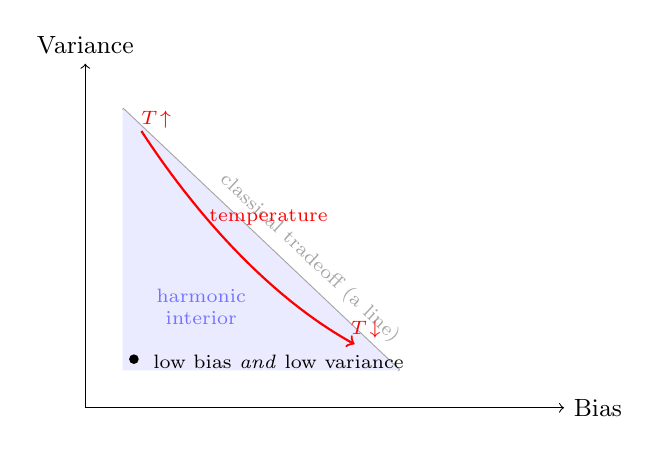
\begin{tikzpicture}[scale=0.95]
        % Axes: bias (x) vs variance (y)
        \draw[->] (0,0) -- (6.4,0) node[right,font=\small] {Bias};
        \draw[->] (0,0) -- (0,4.6) node[above,font=\small] {Variance};

        % Classical tradeoff: a line you must sit on
        \draw[thick,gray!70] (0.5,4.0) -- (4.2,0.5);
        \node[gray!70,font=\scriptsize,rotate=-43] at (3.0,2.0) {classical tradeoff (a line)};

        % Harmonic interior: region reachable when the axes decouple
        \fill[blue!8] (0.5,0.5) -- (4.2,0.5) -- (0.5,4.0) -- cycle;
        \node[blue!55,font=\scriptsize,align=center] at (1.55,1.35) {harmonic\\interior};

        % The desirable corner
        \draw[fill=black] (0.65,0.65) circle (1.6pt);
        \node[font=\scriptsize,right] at (0.78,0.62) {low bias \emph{and} low variance};

        % Temperature dial arrow sweeping into the interior
        \draw[->,red,thick] (0.75,3.7) .. controls (1.6,2.4) and (2.6,1.4) .. (3.6,0.85);
        \node[red,font=\scriptsize] at (2.45,2.55) {temperature};
        \node[red,font=\scriptsize] at (0.95,3.85) {$T\!\uparrow$};
        \node[red,font=\scriptsize] at (3.75,1.05) {$T\!\downarrow$};
    \end{tikzpicture}
    \caption{Bias and variance as orthogonal coordinates. Classically a model must sit somewhere on the gray line: less of one means more of the other. When a static spectrum supplies bias and an input-conditional modulation supplies variance, the two decouple, and the interior (shaded) becomes reachable - lower bias \emph{and} lower variance than any point on the line. Temperature is a path through this space, not noise added at a fixed point.}
    \label{fig:manifold}
\end{figure}

\section{Harmonic Latent Space}
\label{sec:harmonic}

% Gated subsections injected by praxis/pillars/build.py. The first is section 3.1,
% chosen by codec_mode (CALM / byte-latent / standard tokenization) for the run;
% the rest (crystal head, attention sink, the seed) follow by order.
\paperFramingHarmonic

\subsection{The outer representation}

There is a third way to read what this architecture trains for, orthogonal to the bias-variance manifold and to the Koopman dynamics: not \textit{how} it represents, but \textit{where in the sequence the learning pressure falls}. A standard causal model carries a next-token objective at every position; it learns the running interior, the representation as it unfolds one step at a time. A masked model hides interior positions and learns to fill them in; it learns the inner representation by infilling. Both place their pressure inside the window. The harmonic codec places it at the \textit{ends}.

Two objectives sit at the two temporal extremes of a patch. The codec is an autoencoder over $K$ contiguous tokens (\texttt{calm-d}: $K=8$; the plain byte profile, $K=16$): it \textit{reconstructs} the patch it has already consumed, a $K$-scaled cross-entropy that anchors the already-observed - the past, relative to the decision boundary. It does so over a separable harmonic basis that keeps only the lowest total-frequency modes, so smooth-across-patch structure compresses into few coefficients and the cost of holding a patch falls as $K$ grows rather than rising. The outer decoder then \textit{predicts} the next latent, $z_p \mapsto z_{p+1}$, which decodes to the unobserved next patch - the future, $T{+}1$ tokens ahead. One loss reconstructs what is behind the boundary; the other predicts what is in front of it. The interior of the patch is never a target in itself - it is reconstructed only as a by-product of pinning both ends.

The two attention sinks of Section~\ref{sec:definitions} mirror the two objectives in the same geometry. Ghostmax is a zero sink at the head of every attention row - positionless, always reachable, the place a query falls back to when the past holds nothing it needs. Dropoff, when enabled, is a zero sink at the tip - positioned, on the most recent token, the place that forces a query off the easiest signal so it cannot simply copy the present. A sink that absorbs at the start and a sink that injects at the end: together they pull the model toward the boundaries of what it can see and away from the comfortable middle. We call the result the \textit{outer representation} - the model is incentivized at the head and the tail, the edges of the window, rather than along its interior. It is the complement of both standard regimes (Figure~\ref{fig:masks}): causal learning is interior-running, masked learning is interior-filling, and this learns the rim.

\begin{figure}[t]
  \centering
  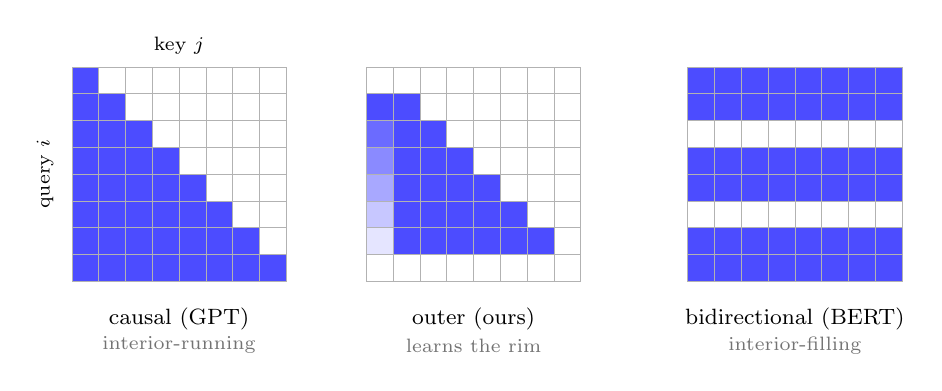
\begin{tikzpicture}[x=0.34cm, y=0.34cm]
    \tikzset{
      attend/.style={fill=blue!70},
      masked/.style={fill=white},
      cb/.style={draw=black!30, line width=0.2pt},
    }
    % ===== Panel 1: causal =====
    \begin{scope}
      \foreach \r in {0,...,7}{
        \foreach \c in {0,...,7}{
          \ifnum\c>\r \fill[masked] (\c,-\r) rectangle (\c+1,-\r-1);
          \else \fill[attend] (\c,-\r) rectangle (\c+1,-\r-1);\fi
          \draw[cb] (\c,-\r) rectangle (\c+1,-\r-1);
        }
      }
      \node[font=\scriptsize,rotate=90] at (-1.0,-4.0) {query $i$};
      \node[font=\scriptsize] at (4.0,0.8) {key $j$};
      \node[font=\footnotesize] at (4.0,-9.4) {causal (GPT)};
      \node[font=\scriptsize,text=black!55] at (4.0,-10.4) {interior-running};
    \end{scope}
    % ===== Panel 2: outer (ours) =====
    \begin{scope}[shift={(11,0)}]
      \foreach \r in {0,...,7}{
        \foreach \c in {0,...,7}{
          \ifnum\r=0 \fill[masked] (\c,-\r) rectangle (\c+1,-\r-1);
          \else
            \ifnum\r=7 \fill[masked] (\c,-\r) rectangle (\c+1,-\r-1);
            \else
              \ifnum\c>\r \fill[masked] (\c,-\r) rectangle (\c+1,-\r-1);
              \else
                \ifnum\c=0
                  \pgfmathtruncatemacro{\shade}{round((6-\r)/5*60+10)}
                  \fill[blue!\shade] (\c,-\r) rectangle (\c+1,-\r-1);
                \else \fill[attend] (\c,-\r) rectangle (\c+1,-\r-1);\fi
              \fi
            \fi
          \fi
          \draw[cb] (\c,-\r) rectangle (\c+1,-\r-1);
        }
      }
      \node[font=\footnotesize] at (4.0,-9.4) {outer (ours)};
      \node[font=\scriptsize,text=black!55] at (4.0,-10.4) {learns the rim};
    \end{scope}
    % ===== Panel 3: bidirectional (BERT) =====
    \begin{scope}[shift={(23,0)}]
      \foreach \r in {0,...,7}{
        \foreach \c in {0,...,7}{
          \fill[attend] (\c,-\r) rectangle (\c+1,-\r-1);
          \draw[cb] (\c,-\r) rectangle (\c+1,-\r-1);
        }
      }
      \foreach \r in {2,5}{
        \foreach \c in {0,...,7}{
          \fill[masked] (\c,-\r) rectangle (\c+1,-\r-1);
          \draw[cb] (\c,-\r) rectangle (\c+1,-\r-1);
        }
      }
      \node[font=\footnotesize] at (4.0,-9.4) {bidirectional (BERT)};
      \node[font=\scriptsize,text=black!55] at (4.0,-10.4) {interior-filling};
    \end{scope}
  \end{tikzpicture}
  \caption{Where the learning pressure falls, read as an attention mask (rows = query position $i$, columns = key position $j$; a blue cell means $i$ attends to $j$). \textbf{Causal (GPT)} is lower-triangular: every position predicts the next from its past, so pressure runs along the interior. \textbf{Bidirectional (BERT)} is the full square with a few interior query rows held out as masked targets (the white bands): pressure fills the interior. \textbf{Outer (ours)} keeps the causal triangle but drops the first and last query rows to sinks - ghostmax at the head, dropoff at the tail - so the objective is anchored at the edges of the window rather than its middle: it learns the rim.}
  \label{fig:masks}
\end{figure}

Pushed one step further - and now firmly into conjecture - the same machinery suggests a regime in which the model \textit{mostly does not transform at all}. A head that falls silent through its ghost is an identity on the residual stream, contributing nothing; and with the input-conditional delta held small against the standing static baseline (Section~\ref{sec:manifold}), the field a sequence sees is dominated by the input-\textit{independent} corpus rhythm. The transform is then nearly the same for every input, and what separates one sequence from another is a sparse scatter of large deviations on a shared standing shape - the smoothness prior carrying that shape forward, each feature entering with a velocity and only now and then kicked off it. Read this way the computation is \textit{event-driven} rather than a fresh dense map at every step, closer in spirit to the sparse activity of spiking systems - a point of contact with biological plausibility we flag as motivation, not as a claim that the architecture is neural. It is checkable in diagnostics already reported: \texttt{harmonic\_delta\_norm} measures how much deviation is added, and how \textit{concentrated} that deviation is across positions and features is the sparsity this reading predicts - a diffuse delta would refute it. It leaves open the further question, which we do not attempt here, of whether a downstream consensus (the CALM vote) could itself raise such events and fold them back into the field.

This is the least settled part of the picture, and we mark the seam honestly. The reconstruction-and-prediction duality is in production and measurable - reconstruction fidelity and the conditional gap between marginal and conditional next-latent prediction are both reported. The outer-representation reading, and the dropoff sink that would complete its symmetry, are a conjecture: the claim that learning pressure migrates to earlier positions is exactly what a measurement of attention mass would confirm or refute. We offer the axis as a third coordinate to look along, not yet as one we have surveyed.

\section{The Scaling Conjecture}
\label{sec:scaling}

\subsection{The watch}

Hold the title literally for a moment. A watch is a mechanism of intricate, meshed gears, and what makes it a watch is that the gears turn \textit{in unison}. Drive one and you drive them all, because the teeth couple them into a single body. Now try to run the watch by turning each gear in sequence - one at a time, the rest held still. You cannot. The logic does not merely become inefficient; it stops being a watch. The architecture, the mesh itself, forbids sequential operation. The coupling is the whole point.

Autoregressive consensus modeling is the attempt to turn the gears in sequence. It emits one position, conditions on it to emit the next, and accumulates the answer a tooth at a time. For a coupled system this is the wrong shape of computation, and its cost is the cost of enumeration: linear in the parts.

The harmonic field turns the gears in unison. The frozen Weyl phases are the teeth - the coupling, cut once and never re-cut, that ties every feature to every position in fixed relation. The amplitude grid is the single mainspring. One inverse transform releases it, and the entire field, every $(t,d)$ cell at once, assumes its shape in a single coupled motion rather than a loop over positions. That is the mechanical content of ``logarithmic'': the whole mechanism moves together, so the cost tracks the number of independent rhythms it carries, not the number of positions it must cover.

And the field is \textit{rebuilt}, not advanced. With input-conditional amplitudes it is re-derived from the input rather than carried forward and nudged; in the limit, the entire shape is reconstructed at every decision boundary, all of them, the whole computation re-formed around the present input. What the model learns under the smoothness prior - which asks the field at one position to predict the field at the next - is not a sequence of outputs but \textit{the ability to hold a shape over time}: to keep the gears meshed, to keep the watch a watch, while the hands sweep. The frozen phases protect the coupling; the smoothness prior protects the form.

This is why the geometric framing is not ornament. Nearly anything we can imagine can be written as a shape - a configuration in some space, a standing wave, a mesh of constraints that must move together or not at all. A model that builds shapes and protects them over time models that structure directly, in unison, where a model that enumerates is forever turning one gear and hoping the rest follow. There is something here, and the rest of this section is an attempt to say how much.

% Gated extension (recurrent mode) injected by praxis/pillars/build.py.
\paperFramingScaling

\subsection{Linear consensus, logarithmic interference}

Here is the claim the rest of the paper has been building toward, stated as a conjecture because that is what it is.

A model that represents its corpus as a \textit{mean} - a consensus, an average of examples - must spend resources roughly in proportion to the number of distinct patterns it needs to express. To hold $N$ patterns it allocates capacity that grows with $N$. This is the linear regime, and it is consistent with why scaling laws ask for ever more parameters and tokens to buy each further increment of capability~\cite{kaplan2020}.

A model that represents its corpus as \textit{interference} - a superposition of $K$ frequency components - addresses a combinatorially larger space. $K$ components with learnable amplitudes and frozen, equidistributed phases produce a field whose distinguishable configurations grow exponentially in $K$, because it is the \textit{pattern of constructive and destructive interference} across components that carries information, not the components individually. To express $N$ configurations you need on the order of $\log N$ components. This is the logarithmic regime. The same asymmetry shows up in time: the transform that builds the field is $O(n \log n)$, and a single transform realizes the whole interference pattern at once rather than enumerating its parts.

\begin{figure}[ht]
    \centering
    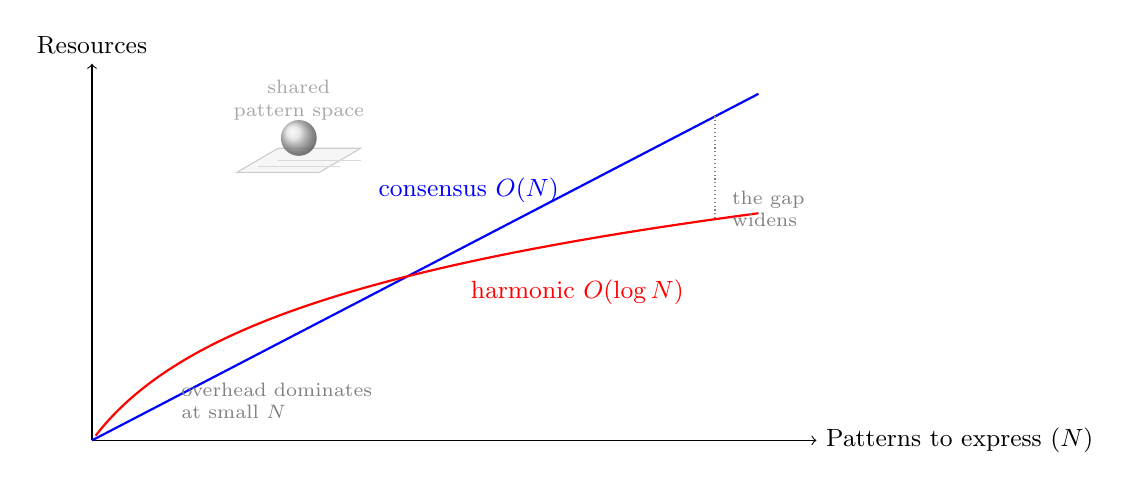
\begin{tikzpicture}[scale=0.92]
        % Axes
        \draw[->] (0,0) -- (10,0) node[right,font=\small] {Patterns to express ($N$)};
        \draw[->] (0,0) -- (0,5.2) node[above,font=\small] {Resources};

        % Consensus / mean: linear O(N)
        \draw[thick,blue,domain=0:9.2,smooth,samples=60] plot (\x,{0.52*\x});
        \node[blue,font=\small] at (5.2,3.45) {consensus $O(N)$};

        % Harmonic / interference: logarithmic O(log N)
        \draw[thick,red,domain=0.05:9.2,smooth,samples=120] plot (\x,{1.35*ln(\x+1)});
        \node[red,font=\small] at (6.7,2.05) {harmonic $O(\log N)$};

        % The widening gap at scale
        \draw[densely dotted,gray] (8.6,{0.52*8.6}) -- (8.6,{1.35*ln(9.6)});
        \node[gray,font=\scriptsize,align=left,right] at (8.7,3.2) {the gap\\widens};

        % small-N note: harmonic overhead
        \node[font=\scriptsize,gray,align=left] at (2.55,0.55) {overhead dominates\\at small $N$};

        % Shared pattern space: the convergence motif (isometric plane + sphere)
        \begin{scope}[xshift=2.0cm,yshift=3.7cm,scale=0.95]
            \fill[gray!12,opacity=0.6] (0,0) -- (1.2,0) -- (1.8,0.35) -- (0.6,0.35) -- cycle;
            \draw[gray!40,thin] (0,0) -- (1.2,0) -- (1.8,0.35) -- (0.6,0.35) -- cycle;
            \draw[gray!30,very thin] (0.3,0.088) -- (1.5,0.088);
            \draw[gray!30,very thin] (0.6,0.175) -- (1.8,0.175);
            \shade[ball color=gray!30,opacity=0.85] (0.9,0.5) circle (0.26);
            \node[gray!70,font=\scriptsize,align=center] at (0.9,1.05) {shared\\pattern space};
        \end{scope}
    \end{tikzpicture}
    \caption{Conjectured scaling regimes. To express $N$ patterns, consensus modeling - learning the mean - spends resources growing linearly in $N$ (blue). Harmonic modeling composes patterns by interference, and $K \sim \log N$ components suffice, so its cost grows logarithmically (red). The harmonic basis carries fixed overhead, so it loses at small $N$ and wins at scale, where the gap widens without bound. Both must ultimately represent the same target (the shared pattern space, top); the claim is about the cost of getting there, not the destination. This figure states a conjecture, and replaces the speculative measured-curve figure of earlier drafts.}
    \label{fig:scaling}
\end{figure}

\subsection{The exponential edge}

Why should a learned network be able to live in the interference regime at all? Because the transformer already computes on an exponential substrate. Every attention layer is a softmax, $\exp(\cdot)/\sum\exp(\cdot)$, which amplifies small differences and converts addition into multiplication; the network is kept numerically alive only by normalization holding activations in the narrow band where the exponential is both sensitive and stable. Euler's identity, $e^{i\pi} = -1$, ties that exponential directly to periodic structure, which is why a harmonic field seeded with $\pi$ and $e$ is not an arbitrary choice of decoration but a resonance with the machinery already present. The harmonic head writes interference patterns onto a substrate that was always exponential; it makes explicit a structure the softmax was implicitly using.

\subsection{Tractability is observer-relative}

If interference lets a model represent exponentially many configurations with logarithmically many components, then a search that is combinatorial when enumerated becomes, in this representation, the reading-off of an interference pattern computed in a single transform. The hardness did not vanish. It moved into the choice of basis. And that relocation is the real claim, which we will state without hedging: in a continuous, nested representational space, $P$ and $NP$ are not two discrete bins a problem falls into once and for all. They are the ends of a spectrum, and where a given instance sits on that spectrum is set by the representation doing the solving - by the observer.

This is the same thesis the rest of the paper has been making, carried to its conclusion. If attention constructs which patterns manifest (Section~\ref{sec:constructor}), and if the basis a model occupies decides whether a structure costs linear or logarithmic resources to express (Figure~\ref{fig:scaling}), then ``intractable'' cannot be a property of the problem alone. It is a property of the pairing between a problem and a solver. The instance that is exponential to one architecture - one that can only enumerate, that holds no basis in which the instance is smooth - is approximable in near-constant work by another that happens to carry the right harmonic. Some observers are simply better at collapsing $NP$-shaped problems toward $P$; others are blocked, not by the problem, but by their own architecture, perspective, or alignment. The watchmaker who cannot perceive the gear cannot build the watch, however long he is given. The difficulty was never only in the watch.

We keep exactly one boundary, and we keep it because it sharpens the claim rather than softening it. This is not a statement about the formal worst-case question - whether the classes $P$ and $NP$ coincide over all inputs and all machines~\cite{cook1971}. That question is deliberately indifferent to who is asking; it abstracts the observer away on purpose. The claim here is the complementary one, and abstracting the observer away is precisely what it refuses to do: for the bounded, structured, approximate problems that real minds and real models actually face, tractability is observer-relative, continuous, and movable - and moving it is what changing your representation \textit{is}. The weak, measurable form is already in the framework: for a family of problems one can record the scaling slope each architecture buys, and watch a single instance migrate along the $P$-to-$NP$ spectrum as the basis changes underneath it.

\section{The Praxis Framework}
\label{sec:framework}

Praxis~\cite{praxis2025} is a registry-based framework in which every component - encoder, decoder, attention, optimizer, loss, router, embedding, head, memory - is swappable, and new implementations become available through registration without touching core infrastructure. Read in light of the preceding sections, its components are not an arbitrary catalogue; each one shapes the representational geometry in a different way, and the framework's purpose is to let those geometries be combined and compared rather than to scale any one of them.

\begin{itemize}[noitemsep]
    % Component-specific bullets enabled per current run by praxis/pillars/build.py;
    % the always-applicable bullets below stay static (and keep the list non-empty).
    \paperFramingFramework
    \item \textbf{Reversible residuals}~\cite{gomez2017reversible} require invertibility throughout the forward pass, forbidding destructive compression and so forcing reconstruction-preserving representations.
    \item \textbf{Attention variants} (multi-head, sliding-window, gated, structured $O(n\cdot c)$, and others) each impose a different relational geometry on the sequence.
    \item \textbf{Mixture-of-experts routing}~\cite{shazeer2017outrageously} and \textbf{tool integration} let several geometries coexist and let external, bias-free computation enter the loop.
\end{itemize}

The configuration hierarchy (Environments $>$ CLI $>$ Experiments $>$ Defaults) makes arbitrary combinations reproducible: different attention per expert, optimizers per layer, frequency offsets~\cite{time2vec2019,tancik2020} per head. \paperRunsLogged{} training runs are documented in the run history. This paper does not present a benchmark table, by design: the framework is the instrument, and the experiment that matters is the one the reader runs to test the scaling conjecture for themselves.

\section{Attention as a Constructor}
\label{sec:constructor}

The framing that motivates all of this is older than the harmonic head. Across physics and neuroscience, observation appears to participate in what is observed rather than passively recording it: measurement affects the quantum system~\cite{heisenberg1927uncertainty}, attention modulates cortical responses to identical stimuli~\cite{treue1996attentional,kastner2000mechanisms}, and predictive-processing accounts make perception an attention-weighted construction rather than a bottom-up readout~\cite{friston2010free,clark2013whatever}. If attention constructs which patterns manifest rather than filtering pre-existing ones, then architectural diversity in attention is not a tuning detail; it determines what is learnable at all.

% Gated paragraph (prismatic head) injected by praxis/pillars/build.py.
\paperFramingConstructor

The measurement analogy invites a sharper question than the one it usually settles for: if observation participates in the observed, does \textit{our} act of observing the model - snapshotting its spectrum, sampling its state - change what it learns? The quantum reading is metaphor, and we keep it as such. But a harmonic field is a standing wave over the full (position, feature) computation, and therefore non-local: a perturbation injected at one cell rides the field to the rest rather than staying put. So a harmonic model should be \textit{more} sensitive to impure observation than one whose features are independent, and the weak, measurable form of the question follows directly. Three of its artifacts are mundane and real. First, a measurement that mutates state rather than reading it purely is a literal observer effect - we have already seen one, where a background thread flipped the model's train/eval flag mid-forward and changed gradients that gate on it; harmonics propagate such a perturbation instead of localizing it. Second, observation forces dtype boundaries a pure forward pass avoids (snapshots cast; the inverse transform is sensitive in its low-order bits), and on the exponential edge of Section~\ref{sec:scaling} rounding can amplify rather than wash out - precisely where the field is most plastic. Third, the run writes records of itself into its own training distribution. At launch the framework renders the model's blueprint to the terminal on a time-ramped curve and stamps the elapsed wall-clock as a rate - a number set by disk caches, scheduler jitter, and thermal state, not by the seed - and rewrites the LICENSE copyright line with the instant of observation expressed as a fractional year (\texttt{\paperLicenseEpoch} at this build), which is then committed. Because the repository is part of the corpus the model trains on, the model ingests the timestamps of its own observations: running the experiment edits the experiment's data. The first two artifacts are testable as a diff between a watched run and an unwatched one from the same seed, against a non-harmonic control that isolates the field's non-locality. The third qualifies what ``unwatched'' can mean: the two arms can never share execution timing, so the complete control is a deterministic, bit-for-bit replay of the entire input timeline - what speedrunners call a tool-assisted run - and anything short of that bounds the effect rather than isolating it. The strong form is the architecture's own: the remote-expert pool the framework runs is, by construction, a passive observer of the model's batches whose gradients never return, so drawing that single coupling - observer to participant - is a clean two-arm ablation of whether being watched, when watching also feeds back, changes which patterns manifest.

\section{Discussion}

\subsection{Answering the opening question}

Do you exist in other people's realities the same way you exist in your own? If the geometry of an attention architecture determines which patterns it constructs, then observers running different geometries build different representations from the same input. You exist in your reality through your geometry, and in another's through theirs. This is not solipsism: convergence to a shared pattern space (Figure~\ref{fig:scaling}) says everyone is reaching the same place. It is the \textit{path} that differs - which patterns manifest, in what order, at what cost - and the path is set by architecture.

\subsection{When two observers couple}
\label{sec:coupling}

If a single observer constructs its reality through its geometry, the next question is what happens when two geometries are not merely different but \textit{coupled} - phase-locked to a common rhythm rather than running independently. The harmonic substrate gives a sharp prediction. Two weakly coupled oscillators with nearby natural frequencies lock together, and at the edge of that locking region the system sits near a bifurcation where its response to a small perturbation diverges. A pair tuned to a shared frame is therefore poised to amplify a perturbation of that frame that either alone would miss. Carried to people, this is the everyday report of \textit{feeling watched}: the conjecture is not that there is a new sense, but that coupling is a gain on an old one. The strongest case for a literal channel is adaptive - a prey animal that senses a fixed predatory gaze outlives one that does not, and the payoff is asymmetric enough, a cheap false alarm against a fatal miss, that selection would favor it - but that same asymmetry is also the deflation: error-management logic builds a deliberately biased, hair-trigger detector, fed by a fast subcortical route that tags gaze and looming motion below awareness, and it predicts both the near-universal \textit{experience} and its poor accuracy, a real and adaptive sense that is heightened ordinary perception rather than a new modality. The folk phenomenon is, on the evidence, best explained away - detection collapses to chance once conventional sensory channels are removed and the looking sequence is properly randomized - but the explaining-away has a regime baked into it that the studies never controlled. They pair strangers, who are uncoupled by construction, and they remove the very channel a coupled pair would amplify. The weak, measurable form follows directly, and it dissociates the two readings: stratify pairs by a measured synchrony index (interpersonal neural and physiological entrainment are now routinely recorded), and cross coupling with sensory isolation. If detection rises with coupling \emph{only} while a conventional channel is open, and vanishes under isolation even for the most synchronized pairs, then the effect is a resonance gain on ordinary cues - the same diverging susceptibility this paper invokes near criticality elsewhere - and nothing exotic is required; if it instead survives isolation, the claim is extraordinary and belongs to a pre-registered replication, not to this paragraph. As with the model's observer effect (Section~\ref{sec:constructor}), the quantum reading is metaphor we do not cash, and the engaged-versus-passive distinction is the same one the framework already runs: a watcher coupled into the frame is the human face of drawing the passive observer pool back into the forward.

\subsection{A note on reconciliation}

The same convergence principle drives the author's companion infrastructure project, Platformer~\cite{platformer2025}, where the explicit design stance is eventual consistency: rather than seeking perfect synchronization, the system runs repeated reconciliation cycles that drift toward a declared desired state and ``find balance'' through iteration. The shift there from fragmented to unified state is described in the same terms as the shift from sparse to fully-connected networks - more global context yields better optimization. Training is reconciliation of this kind: a model is run against its objective again and again until it settles into an attractor, the way a harmonic field settles onto a corpus rhythm or a codec phase-locks. That the same philosophy organizes both a language model and a fleet of cloud accounts is not a coincidence of the author's taste; it is what convergence under repeated local correction looks like, in whatever substrate.

\subsection{The practitioner as proof}

The blind watchmaker is design without a designer: structure that emerges from a blind, iterative process rather than from foresight. That is what these systems do. No one specifies the spectrum the harmonic field will lock onto, or the geometry the crystal centers will grow into; they emerge from the process, and we read them off afterward. Which raises an honest question about what would even count as proof here. A benchmark number proves that one model beat another on one distribution. It does not establish a claim about regimes of representation. The framework's proof, if it has one, is of a different kind: it is the practice itself. \textit{Praxis} is the Greek word for theory enacted - for doing as a form of knowing. The demonstration on offer is not a leaderboard but a method you can run, whose intuitions arrive only by stepping through it yourself. The name is the argument: the proof is in the doing.

% Real Center-PCA densities read off the live checkpoint - the "read them off
% afterward" above, in silico. For a multi-head model (prismatic4's VEAR crystal
% bank) this renders that run's own heads rather than a cross-run mix; generated
% by praxis/pillars/geometries.py (empty macro on a clean checkout).
\paperGeometryFigure

\subsection{Implications for machine learning}

If bias and variance are separable in a harmonic latent space, then they should be learned as input-dependent functions rather than chosen as a global operating point: the field learns which rhythm matters, the delta learns when and how much to deviate, and no per-experiment hyperparameter mediates the two. If the scaling conjecture holds even partially, then on problems with strong periodic or compositional structure, the right move is to change the basis rather than to add parameters, and the linear and logarithmic regimes should be distinguishable by measuring the slope of coverage against resources. Both are testable in the framework, which is the only reason to state them.

% Gated subsection (remote-expert swarm) injected by praxis/pillars/build.py.
\paperFramingDiscussion

% Collected falsifiable conjectures, generated by praxis/pillars/conjectures.
\paperConjectures

\subsection{Limitations}

We are deliberate about what is and is not established. The bias-variance decoupling is grounded in a running implementation and its diagnostics (concentration, smoothness, delta norm, the spectrum heatmap), but ``orthogonal axes'' is an interpretation of those diagnostics, not a theorem. The scaling conjecture of Figure~\ref{fig:scaling} is a conjecture: the figure draws an asserted relationship, not measured curves, and the honest next step is to measure the slope on tasks of varying combinatorial structure and report where harmonic representations fail to buy it. The observer-relative view of tractability (Section~\ref{sec:scaling}) is a philosophical position, and only its weak form - the scaling slope a given basis buys on a given problem family - is measurable; we make no claim about the formal worst-case $P$ versus $NP$ question, which abstracts the observer away by design. The connection to biological attention remains speculative, and the prismatic asymmetry needs to be shown in silico now that the hand-measured figure is gone. The observer effect of Section~\ref{sec:constructor} is, in its quantum form, an analogy we do not cash; only its weak form is a claim - that impure measurement (state-mutating reads, measurement-induced rounding on the exponential edge, self-ingested execution timestamps) perturbs a non-local harmonic field measurably more than an independent-feature one, and that coupling the framework's passive observer pool back into the forward is a two-arm ablation of being-watched. The temporal artifact in particular is a claim about data provenance, not physics: launch rates and license stamps enter the model as tokens, so ``modeling its own time'' means modeling those tokens, and we make no claim that the field encodes execution timing beyond what is literally written into its corpus. Those are diffs between a watched and an unwatched run, not statements about physics. The coupled-observer extension (Section~\ref{sec:coupling}) - that two phase-locked observers amplify perturbations of the frame they share, of which \textit{feeling watched} is the folk instance - is conjecture in the same spirit: its only measurable form is the synchrony-stratified design that separates a resonance gain on ordinary sensory cues from a non-sensory channel, and we side explicitly with the former, against the latter, pending that experiment. None of these are reasons not to state the ideas; they are the boundary between what we have built and what we are conjecturing, drawn so the reader can attack the right target.

\subsection{A direction: the moving point}

% A forward-looking reflection (praxis/pillars/framing/conclusion-ascent.yml),
% deliberately placed BEFORE the conclusion so the closing argument lands last and
% uninterrupted - this coda is a direction, not part of the sign-off.
% The macro emits a lemma + proof; in this reflective passage the proof's QED
% tombstone reads as out of place, so blank \qedsymbol within this group only
% (the formal sections keep their end-of-proof marks).
\begingroup
\renewcommand{\qedsymbol}{}
\paperFramingConclusion
\endgroup

\section{Conclusion}

% The conclusion's opening is thread data (praxis/pillars/threads/<key>.yml);
% the selected thread's generated thread.tex defines \paperThreadConclusion.
\paperThreadConclusion

\appendix

\section{Current Experiment}
\label{sec:current}

\emph{This appendix is generated.} The figure is built from training logs by \texttt{praxis/pillars/build.py}; the paper itself is a template the tool populates. The chart leads with the most recently launched experiment that has logged validation data, and fixes the y-metric to that run's family - here \paperMetricName{} (\texttt{\paperMetricKey}), as of the last export (\paperUpdated). Only experiments that report the \emph{same} metric are drawn alongside it; the rest are listed as omitted below. This is the smallest living slice of the document: one metric, the current experiment against its compatible predecessors.

\ifx\paperCurrentNote\empty\else
    \par\smallskip\noindent\emph{Note:} \paperCurrentNote
\fi

\begin{figure}[h]
    \centering
    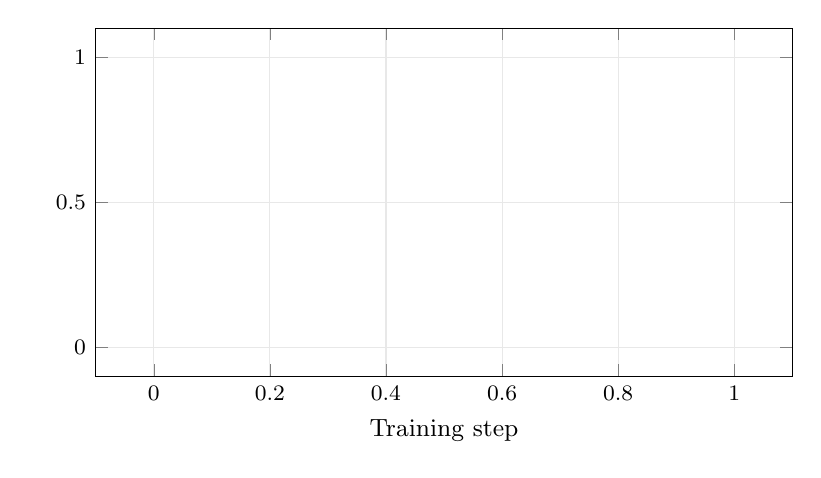
\begin{tikzpicture}
        \begin{axis}[
                width=0.86\linewidth, height=6cm,
                xlabel={Training step}, ylabel={\paperMetricYlabel},
                legend pos=north east, grid=both, grid style={gray!18},
                tick label style={font=\footnotesize}, label style={font=\small},
                legend style={font=\footnotesize, fill opacity=0.85},
            ]
            \paperValPlots
        \end{axis}
    \end{tikzpicture}
    \caption{\paperMetricName{} across the \paperRunCount{} most recent experiments with comparable validation curves; the leading run (\runOneName) is drawn in bold. Generated from run logs - metrics that are not comparable across families (token loss vs.\ byte bits-per-byte vs.\ codec/CALM BrierLM) are excluded by construction, so the curves on this axis mean the same thing.}
    \label{fig:current}
\end{figure}

The current experiment, \runOneName{} (\texttt{\runOneHash}), reached \paperMetricName{} \runOneFinal{} by step \runOneSteps{}. Recent experiments whose families report a different validation metric are omitted rather than plotted on an incomparable axis: \paperSkipped{}.

% Generated table of each recent experiment's training-data mixture
% (praxis/pillars/datasets.py); empty fallback on a clean checkout.
\paperDatasetsTable

% Thread-provided theory components plug in here: the selected thread's
% thread.tex (generated) defines \paperThreadTheory; the empty fallback in
% main.tex omits it. The long-term direction is to migrate the prose above
% into thread components as-data, converging on a thin unified body.
\paperThreadTheory

% Ensure bibliography data is written even if some tools don't see citations
\nocite{*}
{\small
    \bibliographystyle{plain}
    \bibliography{citations}
}

